\subsection{Estimation methods}
% 3 pages
Estimating the extent of tasks is always relevant, as it gives an idea of how long each task probably will take to finish. Even though one does not always actively make these estimations on a small project, one does always have an idea of how long the individual tasks will take.

The knowledge is essential to plan a project because the sum of all estimations sheds light on how long time the project probably will take, which in turn enables several different planning methods to be used, each providing a more-or-less optional route through the tasks.

The use of estimation methods will allow us to be precise and thorough in our estimations. Based on the knowledge acquired from the application of the methods, we are able to make more precise plans to help us overcome the derailed project.

In the following we will present the methods we considered for estimating the tasks of our project, and explain why we choose to use or discard each individual method. For the each chosen method we will also describe how we experienced the use of it.

\subsubsection{Planning Poker}
Multiple estimation methods exists, but for this part of the project we have chosen to use Planning Poker, also know as SCRUM Poker, to estimate our backlog tasks.

Planning Poker seemed like a good choice since we all have worked with SCRUM before, but not used Planning Poker. Now was a great opportunity to practice it.

We think that the fact that the players do not influence each other when estimating, while the game still facilitates shorts discussion, gives Planning Poker an advantage over traditional, discussion-only estimation.
That Planning Poker facilitates discussions is the reason for why we chose Planning Poker over the Delphi estimation method, which does not.

The discussion might not always be an advantage, though. It can easily become very time consuming. We chose a non-voting, but overruling, moderator to address this potential problem, and we believe it worked great proving itself an advantage multiple times.

\begin{figure}[t]
  \centering
  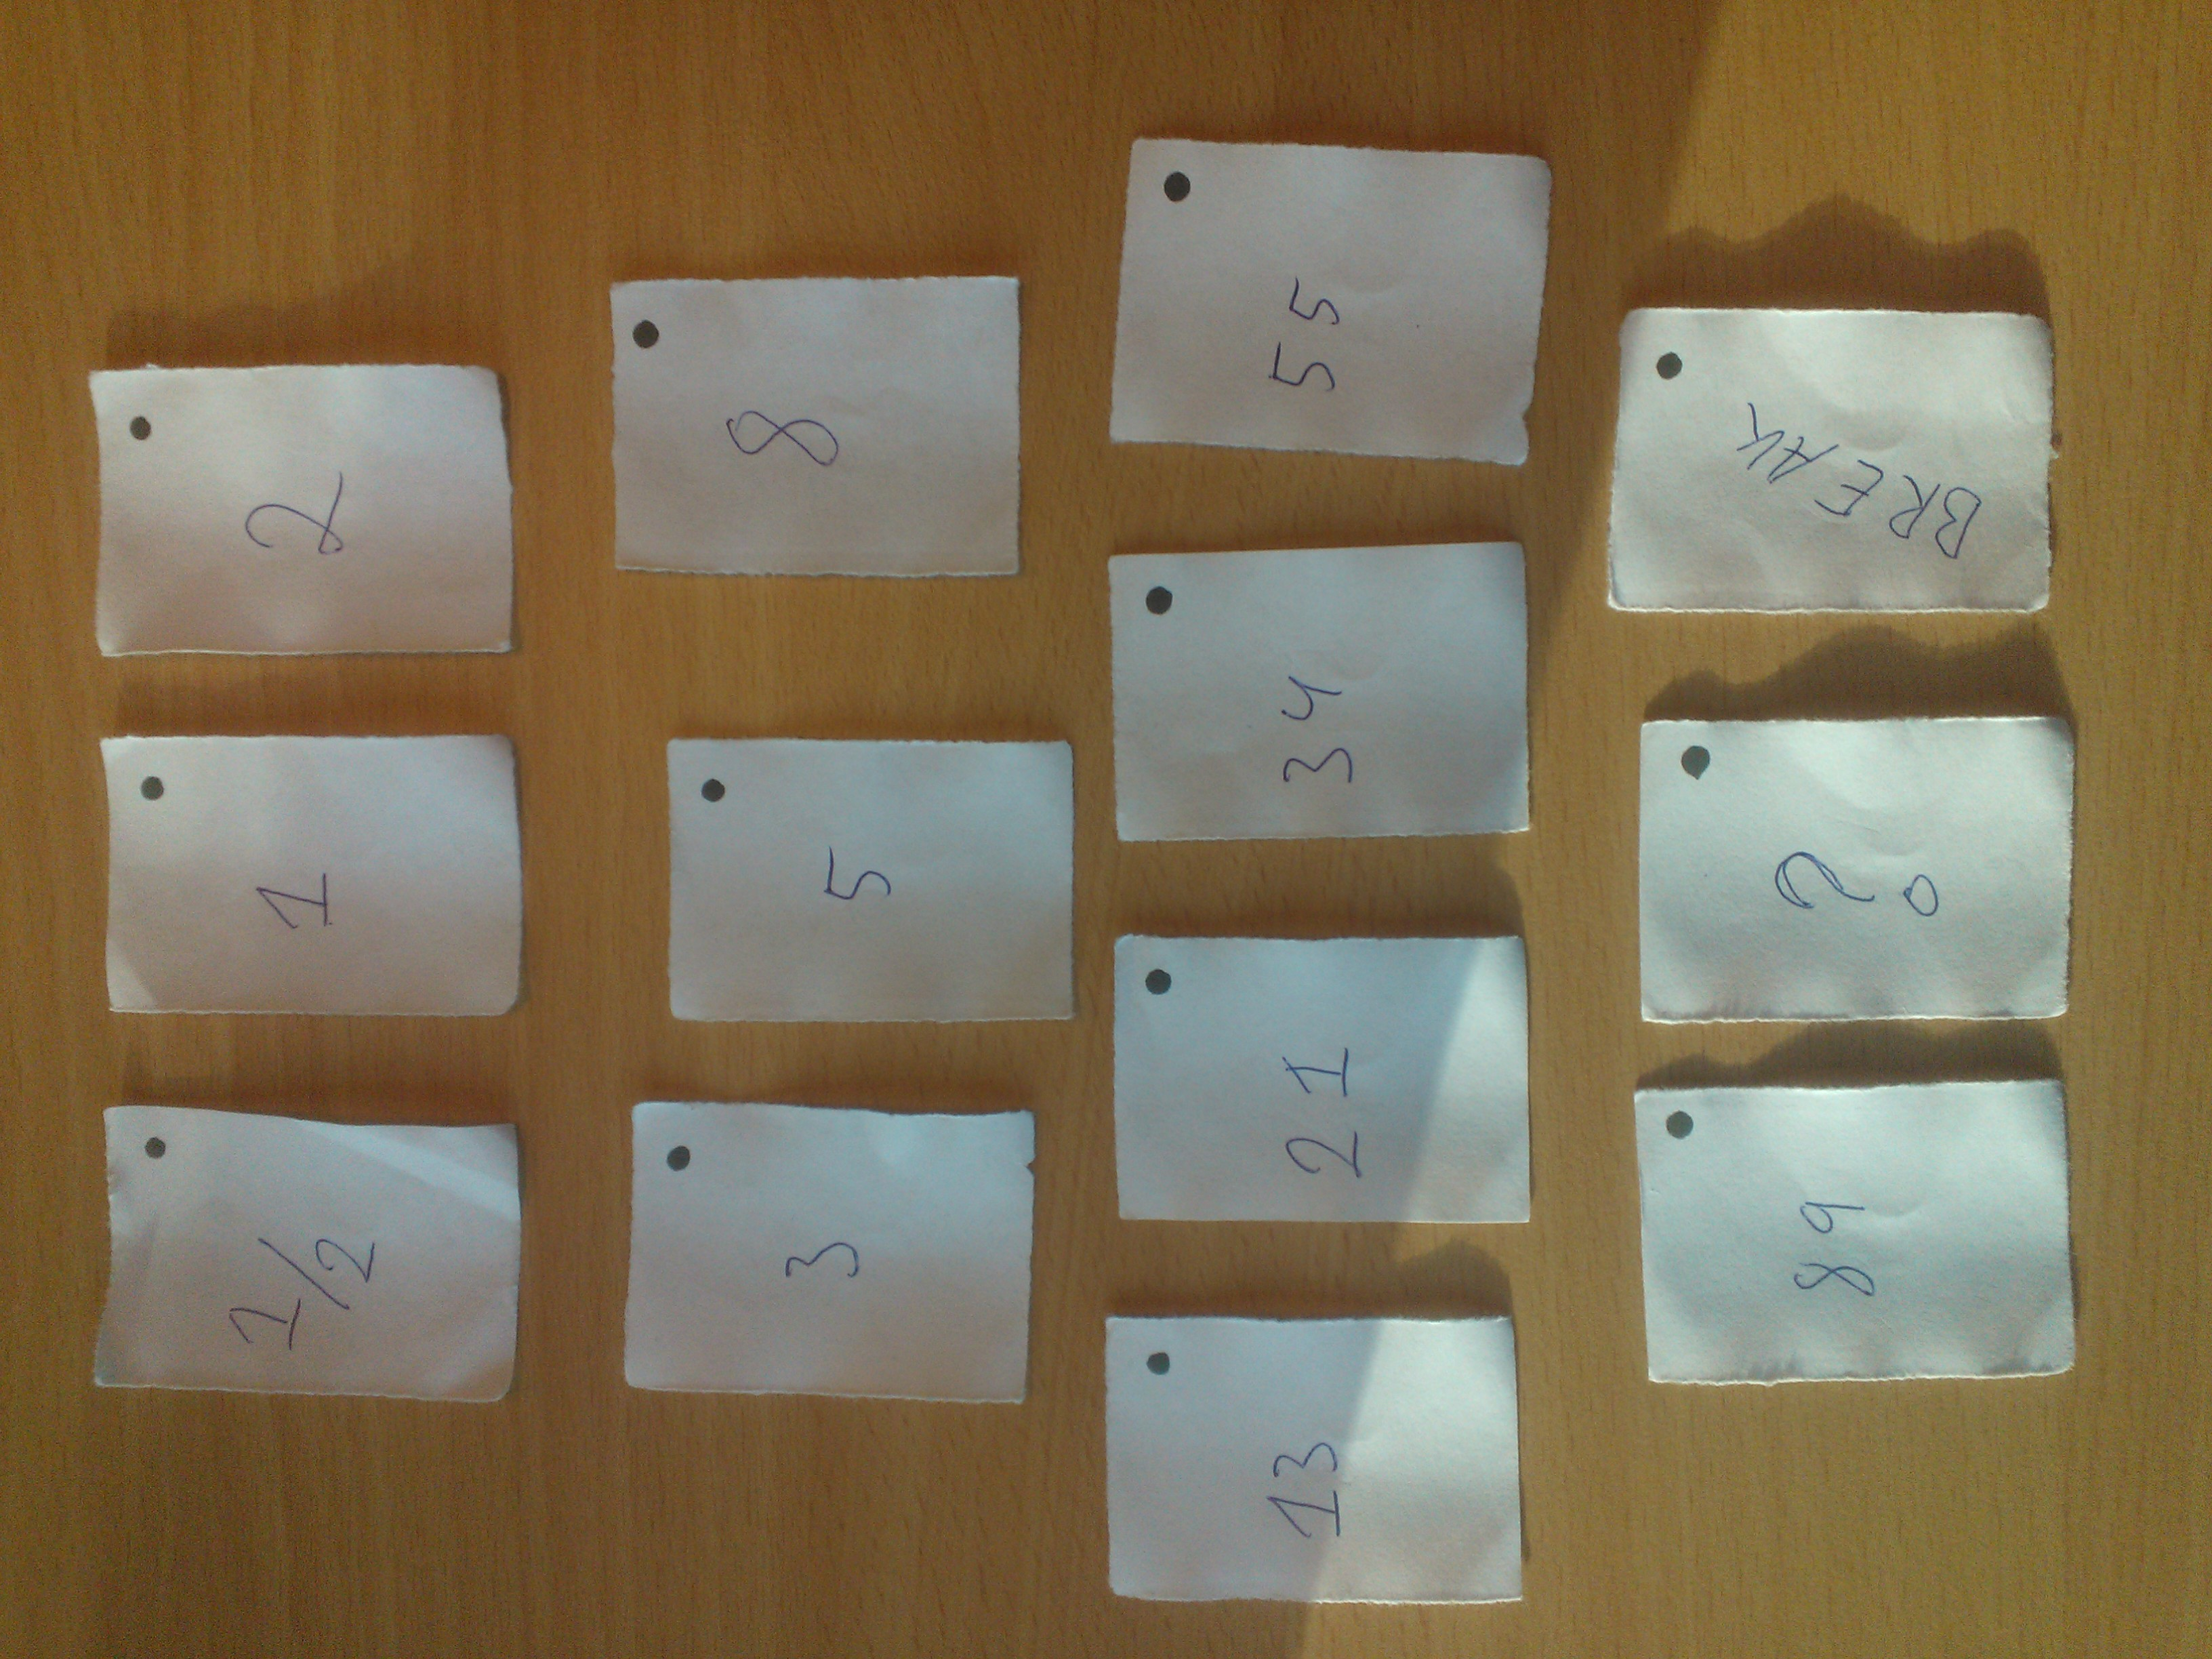
\includegraphics[width=\textwidth, angle=270]{illustrations/scrumPokerCards.jpg}
  \caption{SCRUM Poker cards}
  \label{fig:scrumPokerCards}
\end{figure}

For our game we made playing cards with the numbers 1/2, 1, 2, 3, 5, 8, 13, 21, 34, 55, 89, `?' and `BREAK'. The numbers represented man hours and the question-mark represented that the estimator was unable to give a good estimate, while the `BREAK' card represented that the estimator needed a short break from the game (see figure \ref{fig:scrumPokerCards}).

For this project we found Planning Poker to have several advantages. For one thing, we found it to be way more motivating and pleasing than any other estimation methods we previously have tried. As result all members of the group was kept included in the process, at the same time gaining a better understanding of the tasks as they were discussed.
Second and most important, this time we got a real idea of how much time and effort we should put into each task, in opposite to the results of what we did in the first part of the project.

For our project, however, the high numbers (55 and 89) was never used, and neither was the `break' card. The `?' was only rarely used, but when it was, it introduced weaknesses to the method.
When a person played the card he would not participate in the discussion, which was bad for the quality of the estimation. Worse were when multiple persons played the card, potentially leaving only a single person with a real estimation vote for the task.
At last the card was therefore not considered valid by the team.

\subsubsection{CoCoMo estimation}
CoCoMo is an algorithmic software cost estimation method. With basic CoCoMo one is able to calculate time estimations based on the size of the team, the experience of the team, and the estimated Kilo Lines Of Code (KLOC) to be written factored by the programming language in question.
Estimating all the variables but one, the remaining variable can be calculated, for instance the cost of a project or the team size required for a project. To yield more precise estimations one may expand the CoCoMo calculation model with many more factors, such as complexity, reliability, and hardware constraints, to name a few \cite[p. 147]{PM}.

We have chosen not to use the CoCoMo estimation, since we do not have enough known variables to compute an estimate which is more accurate than using Planning Poker. Had it yielded more accurate results than Planning Poker, it would only have been able to complement it, as CoCoMo does not feature discussion and hence does not provide the benefits stemming from discussion.

\subsubsection{PERT estimation}
The last estimation method we have considered is the PERT estimation method. While most other methods only ends up with one estimation for each task, the PERT method uses three estimates, and then calculate it into one. The force of the PERT method lies in its three estimates \cite[p. 152]{PM}:

It is definitely a possibility to combine the Planning Poker method with the PERT method. Instead of each player only turning one card, each turns three cards: A optimistic estimate, a realistic estimate and a pessimistic estimate. So instead of having to agree on one estimate, the `players' would have to agree on all 3 estimates.

We did not use the PERT-method method (neither the "real" PERT, nor the PERT-Planning-Poker hybrid explained above), due to the fact that we estimated it would take us much longer to make three estimates for each task, than only making one.